\subsection{What is a ring buffer?}\label{what-is-a-ring-buffer}

A ring buffer is a simple, usually fixed-sized, storage mechanism where
contiguous memory is treated as if it is circular, and two index
counters keep track of the current beginning and end of the queue. As
array indexing is not circular, the index counters must wrap around to
zero when moved past the end of the array.\\As data is added (enqueued)
to the front of the queue or removed (dequeued) from tail of the queue,
the current items in the buffer form a train that appears to circle the
track\\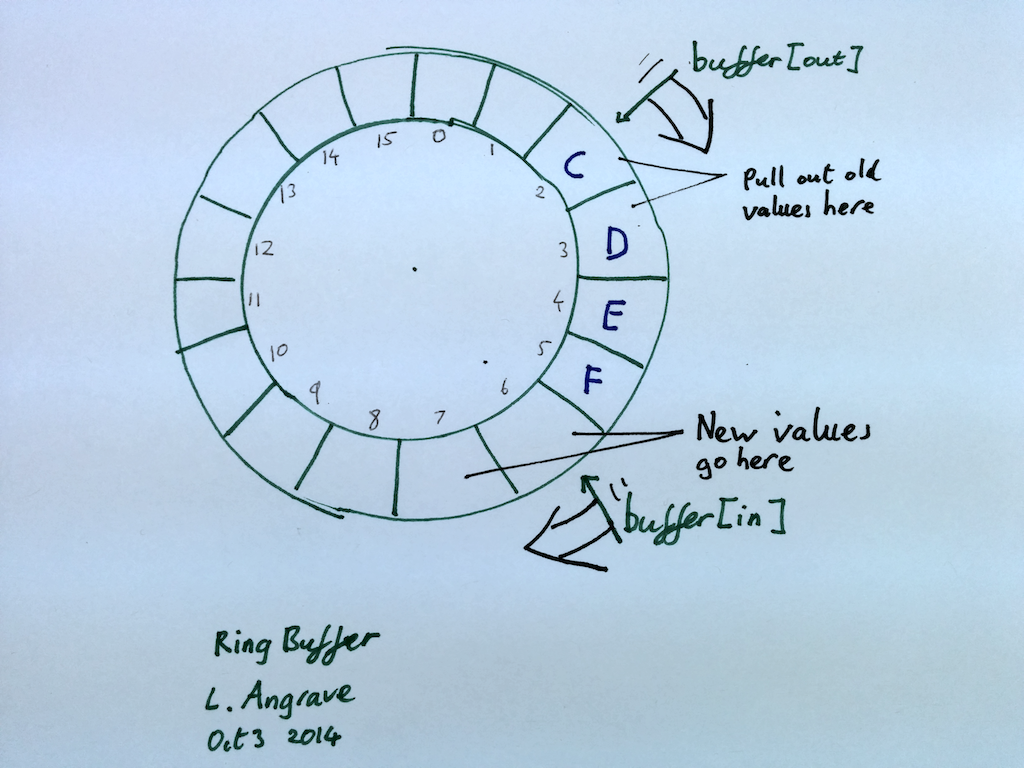
\includegraphics{https://raw.githubusercontent.com/wiki/angrave/SystemProgramming/RingBuffer-Angrave2014-1024x768.png}\\A
simple (single-threaded) implementation is shown below. Note enqueue and
dequeue do not guard against underflow or overflow - it's possible to
add an item when when the queue is full and possible to remove an item
when the queue is empty. For example if we added 20 integers
(1,2,3\ldots{}) to the queue and did not dequeue any items then values
\texttt{17,18,19,20} would overwrite the \texttt{1,2,3,4}. We won't fix
this problem right now, instead when we create the multi-threaded
version we will ensure enqueue-ing and dequeue-ing threads are blocked
while the ring buffer is full or empty respectively.

\begin{Shaded}
\begin{Highlighting}[]
\DataTypeTok{void} \NormalTok{*buffer[}\DecValTok{16}\NormalTok{];}
\DataTypeTok{int} \NormalTok{in = }\DecValTok{0}\NormalTok{, out = }\DecValTok{0}\NormalTok{;}

\DataTypeTok{void} \NormalTok{enqueue(}\DataTypeTok{void} \NormalTok{*value) \{ }\CommentTok{/* Add one item to the front of the queue*/}
  \NormalTok{buffer[in] = value;}
  \NormalTok{in++; }\CommentTok{/* Advance the index for next time */}
  \KeywordTok{if} \NormalTok{(in == }\DecValTok{16}\NormalTok{) in = }\DecValTok{0}\NormalTok{; }\CommentTok{/* Wrap around! */}
\NormalTok{\}}

\DataTypeTok{void} \NormalTok{*dequeue() \{ }\CommentTok{/* Remove one item to the end of the queue.*/}
  \DataTypeTok{void} \NormalTok{*result = buffer[out];}
  \NormalTok{out++;}
  \KeywordTok{if} \NormalTok{(out == }\DecValTok{16}\NormalTok{) out = }\DecValTok{0}\NormalTok{;}
  \KeywordTok{return} \NormalTok{result;}
\NormalTok{\}}
\end{Highlighting}
\end{Shaded}

\subsection{What are gotchas of implementing a Ring
Buffer?}\label{what-are-gotchas-of-implementing-a-ring-buffer}

It's very tempting to write the enqueue or dequeue method in the
following compact form (N is the capacity of the buffer e.g.~16):

\begin{Shaded}
\begin{Highlighting}[]
\DataTypeTok{void} \NormalTok{enqueue(}\DataTypeTok{void} \NormalTok{*value)}
  \NormalTok{b[ (in++) % N ] = value;}
\NormalTok{\}}
\end{Highlighting}
\end{Shaded}

This method would appear to work (pass simple tests etc) but contains a
subtle bug. With enough enqueue operations (a bit more than two billion)
the int value of \texttt{in} will overflow and become negative! The
modulo (or `remainder') operator \texttt{\%} preserves the sign. Thus
you might end up writing into \texttt{b{[}-14{]}} for example!

A compact form is correct uses bit masking provided N is 2\^{}x
(16,32,64,\ldots{})

\begin{Shaded}
\begin{Highlighting}[]
\NormalTok{b[ (in++) & (N}\DecValTok{-1}\NormalTok{) ] = value;}
\end{Highlighting}
\end{Shaded}

This buffer does not yet prevent buffer underflow or overflow. For that,
we'll turn to our multi-threaded attempt that will block a thread until
there is space or there is at least one item to remove.

\subsection{Checking a multi-threaded implementation for correctness
(Example
1)}\label{checking-a-multi-threaded-implementation-for-correctness-example-1}

The following code is an incorrect implementation. What will happen?
Will \texttt{enqueue} and/or \texttt{dequeue} block? Is mutual exclusion
satisfied? Can the buffer underflow? Can the buffer overflow?\\For
clarity \texttt{pthread\_mutex} is shortened to \texttt{p\_m} and we
assume sem\_wait cannot be interrupted.

\begin{Shaded}
\begin{Highlighting}[]
\DataTypeTok{void} \NormalTok{*b[}\DecValTok{16}\NormalTok{]}
\DataTypeTok{int} \NormalTok{in = }\DecValTok{0}\NormalTok{, out = }\DecValTok{0}
\NormalTok{p_m_t lock}
\NormalTok{sem_t s1,s2}
\DataTypeTok{void} \NormalTok{init() \{ }
    \NormalTok{p_m_init(&lock, NULL)}
    \NormalTok{sem_init(&s1, }\DecValTok{0}\NormalTok{, }\DecValTok{16}\NormalTok{)}
    \NormalTok{sem_init(&s2, }\DecValTok{0}\NormalTok{, }\DecValTok{0}\NormalTok{)}
\NormalTok{\}}

\NormalTok{enqueue(}\DataTypeTok{void} \NormalTok{*value) \{}
    \NormalTok{p_m_lock(&lock)}

    \CommentTok{// Hint: Wait while zero. Decrement and return}
    \NormalTok{sem_wait( &s1 ) }
 
    \NormalTok{b[ (in++) & (N}\DecValTok{-1}\NormalTok{) ] = value}

    \CommentTok{// Hint: Increment. Will wake up a waiting thread }
    \NormalTok{sem_post(&s1) }
    \NormalTok{p_m_unlock(&lock)}
\NormalTok{\}}
\DataTypeTok{void} \NormalTok{*dequeue()\{}
    \NormalTok{p_m_lock(&lock)}
    \NormalTok{sem_wait(&s2)}
    \DataTypeTok{void} \NormalTok{*result = b[(out++) & }\DecValTok{15}\NormalTok{]}
    \NormalTok{sem_post(&s2)}
    \NormalTok{p_m_unlock(&lock)}
    \KeywordTok{return} \NormalTok{result}
\NormalTok{\}}
\end{Highlighting}
\end{Shaded}

\subsection{Analysis}\label{analysis}

Before reading on, see how many mistakes you can find. Then determine
what would happen if threads called the enqueue and dequeue methods.

\begin{itemize}
\item
  The enqueue method waits and posts on the same semaphore (s1) and
  similarly with equeue and (s2) i.e.~we decrement the value and then
  immediately increment the value, so by the end of the function the
  semaphore value is unchanged!
\item
  The initial value of s1 is 16, so the semaphore will never be reduced
  to zero - enqueue will not block if the ring buffer is full - so
  overflow is possible.
\item
  The initial value of s2 is zero, so calls to dequeue will always block
  and never return!
\item
  The order of mutex lock and sem\_wait will need to be swapped (however
  this example is so broken that this bug has no effect!)

  \subsection{Checking a multi-threaded implementation for correctness
  (Example
  1)}\label{checking-a-multi-threaded-implementation-for-correctness-example-1-1}
\end{itemize}

The following code is an incorrect implementation. What will happen?
Will \texttt{enqueue} and/or \texttt{dequeue} block? Is mutual exclusion
satisfied? Can the buffer underflow? Can the buffer overflow?\\For
clarity \texttt{pthread\_mutex} is shortened to \texttt{p\_m} and we
assume sem\_wait cannot be interrupted.

\begin{Shaded}
\begin{Highlighting}[]
\DataTypeTok{void} \NormalTok{*b[}\DecValTok{16}\NormalTok{]}
\DataTypeTok{int} \NormalTok{in = }\DecValTok{0}\NormalTok{, out = }\DecValTok{0}
\NormalTok{p_m_t lock}
\NormalTok{sem_t s1, s2}
\DataTypeTok{void} \NormalTok{init() \{}
    \NormalTok{sem_init(&s1,}\DecValTok{0}\NormalTok{,}\DecValTok{16}\NormalTok{)}
    \NormalTok{sem_init(&s2,}\DecValTok{0}\NormalTok{,}\DecValTok{0}\NormalTok{)}
\NormalTok{\}}

\NormalTok{enqueue(}\DataTypeTok{void} \NormalTok{*value)\{}

 \NormalTok{sem_wait(&s2)}
 \NormalTok{p_m_lock(&lock)}

 \NormalTok{b[ (in++) & (N}\DecValTok{-1}\NormalTok{) ] = value}

 \NormalTok{p_m_unlock(&lock)}
 \NormalTok{sem_post(&s1)}
\NormalTok{\}}

\DataTypeTok{void} \NormalTok{*dequeue()\{}
  \NormalTok{sem_wait(&s1)}
  \NormalTok{p_m_lock(&lock)}
  \DataTypeTok{void} \NormalTok{*result = b[(out++) & }\DecValTok{15}\NormalTok{]}
  \NormalTok{p_m_unlock(&lock)}
  \NormalTok{sem_post(&s2)}

  \KeywordTok{return} \NormalTok{result;}
\NormalTok{\}}
\end{Highlighting}
\end{Shaded}

\subsubsection{Analysis}\label{analysis-1}

\begin{itemize}
\itemsep1pt\parskip0pt\parsep0pt
\item
  The initial value of s2 is 0. Thus enqueue will block on the first
  call to sem\_wait even though the buffer is empty!
\item
  The initial value of s1 is 0. Thus dequeue will not block on the first
  call to sem\_wait even though the buffer is empty - oops Underflow!
  The dequeue method will return invalid data.
\item
  The code does not satisfy Mutual Exclusion; two threads can modify
  \texttt{in} or \texttt{out} at the same time! The code appears to use
  mutex lock. Unfortunately the lock was never initialized with
  \texttt{pthread\_mutex\_init()} or
  \texttt{PTHREAD\_MUTEX\_INITIALIZER} - so the lock may not work
  (\texttt{pthread\_mutex\_lock} may simply do nothing)
\end{itemize}

\subsection{Correct implementation of a ring
buffer}\label{correct-implementation-of-a-ring-buffer}

The pseudo-code (\texttt{pthread\_mutex} shortened to \texttt{p\_m} etc)
is shown below.

As the mutex lock is stored in global (static) memory it can be
initialized with \texttt{PTHREAD\_MUTEX\_INITIALIZER}.If we had
allocated space for the mutex on the heap, then we would have used
\texttt{pthread\_mutex\_init(ptr,\ NULL)}

\begin{Shaded}
\begin{Highlighting}[]
\OtherTok{#include <pthread.h>}
\OtherTok{#include <semaphore.h>}
\CommentTok{// N must be 2^i}
\OtherTok{#define N (16)}

\DataTypeTok{void} \NormalTok{*b[N]}
\DataTypeTok{int} \NormalTok{in = }\DecValTok{0}\NormalTok{, out = }\DecValTok{0}
\NormalTok{p_m_t lock = PTHREAD_MUTEX_INITIALIZER}
\NormalTok{sem_t countsem, spacesem}

\DataTypeTok{void} \NormalTok{init() \{}
  \NormalTok{sem_init(&countsem, }\DecValTok{0}\NormalTok{, }\DecValTok{0}\NormalTok{)}
  \NormalTok{sem_init(&spacesem, }\DecValTok{0}\NormalTok{, }\DecValTok{16}\NormalTok{)}
\NormalTok{\}}
\end{Highlighting}
\end{Shaded}

The enqueue method is shown below. Notice,

\begin{itemize}
\itemsep1pt\parskip0pt\parsep0pt
\item
  The lock is only held during the critical section (access to the data
  structure).
\item
  A complete implementation would need to guard against early returns
  from \texttt{sem\_wait} due to POSIX signals.
\end{itemize}

\begin{Shaded}
\begin{Highlighting}[]
\NormalTok{enqueue(}\DataTypeTok{void} \NormalTok{*value)\{}
 \CommentTok{// wait if there is no space left:}
 \NormalTok{sem_wait( &spacesem )}

 \NormalTok{p_m_lock(&lock)}
 \NormalTok{b[ (in++) & (N}\DecValTok{-1}\NormalTok{) ] = value}
 \NormalTok{p_m_unlock(&lock)}

 \CommentTok{// increment the count of the number of items}
 \NormalTok{sem_post(&countsem)}
\NormalTok{\}}
\end{Highlighting}
\end{Shaded}

The \texttt{dequeue} implementation is shown below. Notice the symmetry
of the synchronization calls to \texttt{enqueue}. In both cases the
functions first wait if the count of spaces or count of items is zero.

\begin{Shaded}
\begin{Highlighting}[]
\DataTypeTok{void} \NormalTok{*dequeue()\{}
  \CommentTok{// Wait if there are no items in the buffer}
  \NormalTok{sem_wait(&countsem)}

  \NormalTok{p_m_lock(&lock)}
  \DataTypeTok{void} \NormalTok{*result = b[(out++) & (N}\DecValTok{-1}\NormalTok{)]}
  \NormalTok{p_m_unlock(&lock)}

  \CommentTok{// Increment the count of the number of spaces}
  \NormalTok{sem_post(&spacesem)}

  \KeywordTok{return} \NormalTok{result}
\NormalTok{\}}
\end{Highlighting}
\end{Shaded}

\subsection{Food for thought}\label{food-for-thought}

\begin{itemize}
\itemsep1pt\parskip0pt\parsep0pt
\item
  What would happen if the order of \texttt{pthread\_mutex\_unlock} and
  \texttt{sem\_post} calls were swapped?
\item
  What would happen if the order of \texttt{sem\_wait} and
  \texttt{pthread\_mutex\_lock} calls were swapped?
\end{itemize}
